\chapter{Time Series}
\section{Introduction}

\begin{definition}{Time series}{time-series}\index{time-series}
	Ordered sequence of observations of the same phenomenon. Typically
	measured at equally spaced successive instants of time.
	\begin{equation*}
		\{X_t\}_{t=1,\ldots,T} = \{X_1, X_2, \ldots, X_T\}
	\end{equation*}
\end{definition}

\subsection{Motivation}

Describing and forecasting time series is crucial in different areas of
knowledge; including finance, econometrics, signal processing and a long etc.

\subsection{Objectives}

\begin{itemize}
	\item \textbf{Description}: Describe temporal patterns in a time series: regular and/or
	      seasonal effects, cyclicity, trends, outliers, sudden changes, breaks, \dots
	\item \textbf{Estimation}: Estimate the values of the time series parameters.
	\item \textbf{Validation}: Validate the estimated parameters and decide if the estimated
	      parameters are significant or not.
	\item \textbf{Prediction/Forecasting}: Predict future values of the time series.
\end{itemize}

\begin{example}{AirPassengers}{AirPassengers}
	Monthly totals of international airline passengers in USA, 1949
	to 1960 (Box \& Jenkins, 1976).
	\begin{verbatim}
##      Jan Feb Mar Apr May Jun Jul Aug Sep Oct Nov Dec
## 1949 112 118 132 129 121 135 148 148 136 119 104 118
## 1950 115 126 141 135 125 149 170 170 158 133 114 140
## 1951 145 150 178 163 172 178 199 199 184 162 146 166
## 1952 171 180 193 181 183 218 230 242 209 191 172 194
## 1953 196 196 236 235 229 243 264 272 237 211 180 201
## 1954 204 188 235 227 234 264 302 293 259 229 203 229
## 1955 242 233 267 269 270 315 364 347 312 274 237 278
## 1956 284 277 317 313 318 374 413 405 355 306 271 306
## 1957 315 301 356 348 355 422 465 467 404 347 305 336
## 1958 340 318 362 348 363 435 491 505 404 359 310 337
## 1959 360 342 406 396 420 472 548 559 463 407 362 405
## 1960 417 391 419 461 472 535 622 606 508 461 390 432
\end{verbatim}
	\begin{nscenter}
		\begin{tikzpicture}
			\begin{axis}[
					width=0.9\textwidth,
					height=0.4\textwidth,
					date coordinates in=x,
					table/col sep=comma,
					xlabel=Time,
					ylabel=Passengers,
					xticklabel=\year,
					xtick distance=366*2,
					mark size=1pt,
					mark=o,
					xmajorgrids=true,
					minor x tick num=1,
					xminorgrids=true,
				]
				\addplot table[x=Month,y=Passengers] {data/AirPassengers.csv};
			\end{axis}
		\end{tikzpicture}
	\end{nscenter}
\end{example}

\subsection{Exploratory Data analysis}

Plot of the series and identification of the components:

\begin{definition}{Trend ($T_t$)}{trend}\index{trend}
	Long term tendency of the series.

	Moving average of order $s$:
	\begin{equation*}
		T_t = \frac{1}{s} \sum_{i=1}^s X_{t-s/2+i}
	\end{equation*}
\end{definition}

\begin{definition}{Seasonal ($S_t$)}{seasonal}\index{seasonal}
	Pattern repeated periodically with the same period.

	\index{detrended series}
	\paragraph{Seasonal index} Mean for each period of detrended series ($X_t - T_t$).
\end{definition}

\begin{definition}{Cycle ($C_t$)}{cycle}\index{cycle}
	Pattern repeated periodically with \emph{non-constant} period.

	\vspace{1em}
	\begin{marker}
		Not easy to model due to the changing period.
	\end{marker}
\end{definition}

\begin{definition}{Random ($w_t$)}{random}\index{random}
	Random noise.

	\paragraph{Remainder} ($X_t - T_t - S_t - C_t$)
\end{definition}

Our \emph{goal} is to find a mathematical model that reflects the behavior of the observed
data.

\subsection{Modeling}

\subsubsection{Additive model}
We add the different components:\index{additive model}
\begin{equation}
	X_t = T_t + S_t + C_t + w_t \tag{additive}
\end{equation}

\begin{figure}[H]
	\begin{tikzpicture}
		\begin{axis}[
				width=0.9\textwidth,
				height=0.5\textwidth,
				date coordinates in=x,
				xticklabel=\year,
				xtick distance=366*2,
				xlabel=Time,
				ylabel=Passengers,
				ymajorgrids=true,
				yminorgrids=true,
				xmajorgrids=true,
				minor x tick num=1,
				xminorgrids=true,
				legend pos=north west,
			]
			\directlua{dofile("lua/decomposition.lua")}

			\addlegendentry{$X$ (data)}
			\addlegendentry{$T$ (trend)}
			\addlegendentry{$S$ (seasonal)}
			\addlegendentry{$T+S$}
			\addlegendentry{$w = X-T-S$ (random)}
		\end{axis}
	\end{tikzpicture}
	\caption{Decomposition of the \texttt{AirPassengers} series from example~\ref{ex:AirPassengers}}
\end{figure}

\subsubsection{Deterministic model}\index{deterministic model}
The expected value of $X_t$ depends on a parametric function $F$ of $t$ and the random
component does not depend on the previous values.
\begin{equation}
	X_t = F(t) + Z_t \qquad Z_t \sim N(0,\, \sigma_z^2) \tag{deterministic}
\end{equation}

\subsubsection{Stochastic model}\index{stochastic model}
The expected value of $X_t$ depends on the previous values $X_{t-1}, X_{t-2}, \dots$ and/or
the previous random components $Z_{t-1}, Z_{t-2}, \dots$ plus a random component independent
of the past $Z_t$.
\begin{equation}
	X_t = G(X_{t-1}, X_{t-2}, \dots, Z_{t-1}, Z_{t-2}, \dots) + Z_t \qquad Z_t \sim N(0,\, \sigma_z^2) \tag{stochastic}
\end{equation}

\subsection{Box-Jenkins methodology}\index{Box-Jenkins methodology}

\begin{nscenter}
	\begin{tikzpicture}[
			box/.style={draw, rectangle, minimum width=5cm, minimum height=1.5cm, align=center},
			decision/.style={diamond, minimum width=2cm, minimum height=1cm, align=center},
			box_l/.style={align=left},
		]
		\node[box, rounded corners] (ti) {Tentative\\Identification};
		\node[box, below=of ti] (est) {Estimation};
		\node[box, below=of est] (val) {Diagnostic\\ Checking};
		\node[box, decision, below=of val] (dec) {Model\\ok?};
		\node[box, rounded corners, below=of dec] (fin) {Final Model};

		\node[box_l, right=of ti] {Time Series Plot \\Range-Mean Plot\\ACF and PACF};
		\node[box_l, right=of est] {Least Squares or\\Maximum Likelihood};
		\node[box_l, right=of val] {Residual Analysis\\and Forecasts};
		\node[box_l, right=of fin] {Forecasting\\Explanation};


		\draw[->] (ti) -- (est);
		\draw[->] (est) -- (val);
		\draw[->] (val) -- (dec);
		\draw[->] (dec) edge[edge label={Yes}] (fin);

		\coordinate (fb) at ($(val.west)+(-3em,0)$);
		\node (no) at ($(dec.west)+(-2em,0)$) {No};
		\draw[->] (dec.west) -- (no) -| (fb) |- (ti.west);
	\end{tikzpicture}
\end{nscenter}

\subsection{Distribution of a general stochastic process}

First and second moments for the multivariate distribution of $\{X_t\}_{t=1\dots T}$:
\begin{align*}
	\mathbb{E}[(X_1, \dots, X_T)] & = (\mu_1, \dots, \mu_T)                                              \\
	Var[(X_1, \dots, X_T)]        & = \begin{pmatrix}
		                                  \sigma_1^2   & \sigma_{1,2} & \sigma_{1,3} & \dots  & \sigma_{T,1} \\
		                                  \sigma_{2,1} & \sigma_2^2   & \sigma_{2,3} & \dots  & \sigma_{T,2} \\
		                                  \sigma_{3,1} & \sigma_{3,2} & \sigma_3^2   & \dots  & \sigma_{T,3} \\
		                                  \vdots       & \vdots       & \vdots       & \ddots & \vdots       \\
		                                  \sigma_{T,1} & \sigma_{T,2} & \sigma_{T,3} & \dots  & \sigma_T^2
	                                  \end{pmatrix}
\end{align*}

Parameters of the model:
\begin{itemize}
	\item $T$ values for the mean $\mathbb{E}(X_t) = \mu_t$
	\item $T$ values for the variances $Var(X_t) = \sigma_t^2$
	\item $T(T-1)$ values for the covariances $Cov(X_t, X_s) = \sigma_{t,s}$
\end{itemize}

\subsection{Stationary Series}\index{stationary series}

Strict Stationary Process or Series has the following properties:
The joint distribution of the whole series does not depend on the time
origin:
\begin{equation}
	F_{X_1, \dots, X_t}(x_1, \dots, x_t) = F_{X_{1+s}, \dots, X_{t+s}}(x_{1+s}, \dots x_{t+s}) \quad \forall\; t,s
\end{equation}

\subsection{Weakly Stationary process}
The two first moments of the multivariate distribution of the whole series
does not depend on the time origin:
\begin{itemize}
	\item Constant mean $\mu$.
	\item Constant variance $\sigma^2$.
	\item Constant auto-covariance structure $\sigma_{t,s} = \sigma_{\lVert t - s \rVert}$.
	\item The latter refers to the covariance between $X_t$ and $X_{t-1}$ being equal to
	      the covariance between $X_{t-s}$ and $X_{t-s-1}$.
\end{itemize}

Weakly Stationary process + Gaussian multivariate distribution $\Longrightarrow$ Strict Stationary process.

\begin{question}{Is our data stationary? How can we detect?}{}
	\begin{itemize}
		\item Plot the data.
		\item Identify no stationary components (trends, seasonal patterns, cycles).
		\item Transform the series to remove those components.
		\item For the transformed (stationary) series, plot and analyze the sample autocorrelation.
	\end{itemize}
\end{question}

\begin{marker}\index{Non-constant variance}
	It is very common that the variance of the series increases when the level of the series rises.
\end{marker}

\begin{figure}[H]
	\begin{tikzpicture}
		\begin{axis}[
				width=0.48\textwidth,
				height=0.4\textwidth,
				date coordinates in=x,
				table/col sep=comma,
				xlabel=Time,
				ylabel=Passengers,
				xticklabel=\year,
				xtick distance=366*4,
				mark size=1pt,
				mark=o,
				xmajorgrids=true,
				minor x tick num=1,
				xminorgrids=true,
				title={\bfseries Non-Constant Variance},
			]
			\addplot table[x=Month,y=Passengers] {data/AirPassengers.csv};
		\end{axis}
	\end{tikzpicture}
	\begin{tikzpicture}
		\begin{axis}[
				width=0.48\textwidth,
				height=0.4\textwidth,
				table/col sep=comma,
				xlabel=Time,
				ylabel=$\text{CO}_2$ (ppm),
				mark size=1pt,
				mark=o,
				xmajorgrids=true,
				minor x tick num=1,
				xminorgrids=true,
				enlargelimits=false,
				x tick label style={/pgf/number format/.cd, set thousands separator={}},
				title={\bfseries Constant Variance},
			]
			\addplot+[red] table[mark=none,x=decimal date,y=average] {./data/co2_mm_mlo.csv};
		\end{axis}
	\end{tikzpicture}
	\caption{Examples of constant and non-constant variance}
\end{figure}

\pagebreak
\subsection{Tools to diagnose the non-constant variance}

\paragraph{Mean-Variance Plot} Calculate the mean and variance of consecutive
groups of 8-12 observations. Plot the variance against the mean of each group.

\begin{figure}[H]
	\begin{tikzpicture}
		\begin{axis}[
				width=0.9\textwidth,
				height=0.5\textwidth,
				xlabel=Mean,
				ylabel=Variance,
				% ymajorgrids=true,
				% yminorgrids=true,
				% xmajorgrids=true,
			]
			\directlua{dofile("lua/variance-mean.lua")}
		\end{axis}
	\end{tikzpicture}
	\caption{Mean-Variance plot of the \texttt{AirPassengers} series}
\end{figure}

\paragraph{Boxplot for periods} Represent the boxplot for each group of 8-12
observations. The height of the box (IQR) is a robust estimate of variability.

\begin{figure}[H]
	\begin{tikzpicture}
		\begin{axis}[
				width=0.9\textwidth,
				height=0.5\textwidth,
				xlabel=Time,
				ylabel=Passengers,
				% ymajorgrids=true,
				% yminorgrids=true,
				% xmajorgrids=true,
				boxplot/draw direction=y,
				xtick={2,4,6,8,10,12},
				xticklabels={1950,1952,1954,1956,1958,1960},
				% boxplot/median/.style={line width=2pt},
			]
			\directlua{dofile("lua/boxplot.lua")}
		\end{axis}
	\end{tikzpicture}
	\caption{Boxplot for periods of the \texttt{AirPassengers} series}
\end{figure}

\begin{itemize}
	\item If the variance is similar for all the groups $\Longrightarrow$ No scale transformation.
	\item If the variance is higher for higher values of the mean $\Longrightarrow$ Change the scale.
\end{itemize}

\subparagraph{Box-Cox transformation}
Once we have identified a non-constant variance, we apply a scale
transformation to make it constant. For this, we use the Box-Cox:
\begin{equation}
	Y_t = \begin{cases}
		\frac{X_t^\lambda - 1}{\lambda} & \text{if } \lambda \neq 0 \\
		\ln(X_t)                        & \text{if } \lambda = 0
	\end{cases} \qquad \lambda \in [-1,\,2]
\end{equation}
\begin{marker}
	Usually, the logarithmic transformation is used since it easier to interpret.
\end{marker}

\subsection{Seasonal difference}
To diagnose the seasonal pattern, we can use \mintinline{R}{monthplot}
from the \mintinline{R}{forecast} package. Or we can use the \mintinline{R}{ts.plot}. Below we show examples of its usage and their input (recreated in pgfplots with lua)

\begin{minted}{R}
monthplot(log(AirPassengers))
ts.plot(matrix(log(AirPassengers),nrow=12),col=1:8)
\end{minted}

\begin{figure}[H]
	\begin{tikzpicture}
		\begin{axis}[
				width=0.9\textwidth,
				height=0.3\textwidth,
				xlabel=Month,
				ylabel=Passengers (log),
				xtick={1,2,3,4,5,6,7,8,9,10,11,12},
				xticklabels={Jan,Feb,Mar,Apr,May,Jun,Jul,Aug,Sep,Oct,Nov,Dec},
				ymode=log,
			]
			\directlua{dofile("lua/monthplot.lua")}
		\end{axis}
	\end{tikzpicture}
	\begin{tikzpicture}
		\begin{axis}[
				width=0.9\textwidth,
				height=0.3\textwidth,
				xlabel=Month,
				ylabel=Passengers (log),
				xtick={1,2,3,4,5,6,7,8,9,10,11,12},
				xticklabels={Jan,Feb,Mar,Apr,May,Jun,Jul,Aug,Sep,Oct,Nov,Dec},
				ymode=log,
				cycle list name=exotic,
			]
			\directlua{dofile("lua/tsplot.lua")}
		\end{axis}
	\end{tikzpicture}
	\caption{monthplot (top) and ts.plot (bottom) of the \texttt{AirPassengers} series}
\end{figure}

\begin{definition}{Backshift operator}{backshift}
	Same as the lag operator $L$ in some textbooks.
	\begin{equation}
		B^s X_t = X_{t-s} \qquad BX_t = X_{t-1}
	\end{equation}
\end{definition}

\begin{definition}{Moving average of order $s$}{movingaverage}
	\begin{equation}
		W_t = \frac{1}{s} \sum_{i=1}^s X_{t-i+1} = (1 + B + \cdots + B^{s-1}) X_t
	\end{equation}
\end{definition}

\begin{definition}{Seasonal difference of order $s$}{seasonaldifference}
	\begin{equation}
		W_t = X_t - X_{t-s} = (1 - B^s) X_t = \nabla_s X_t
	\end{equation}
	\tcblower
	\begin{note}
		The seasonal difference is the equivalent to a regular difference of a
		moving average of order $s$:
		\begin{equation}
			(1 - B^s) = (1 - B) (1 + B + \cdots + B^{s-1})
		\end{equation}
	\end{note}
\end{definition}

\begin{figure}[H]
	\begin{tikzpicture}
		\begin{axis}[
				width=0.48\textwidth,
				height=0.4\textwidth,
				date coordinates in=x,
				table/col sep=comma,
				xlabel=Time,
				ylabel=Passengers,
				xticklabel=\year,
				xtick distance=366*4,
				xmajorgrids=true,
				minor x tick num=1,
				ymode=log,
				xminorgrids=true,
			]
			\addplot+[mark=none] table[x=Month,y=Passengers] {data/AirPassengers.csv};
		\end{axis}
	\end{tikzpicture}
	\begin{tikzpicture}
		\begin{axis}[
				width=0.47\textwidth,
				height=0.4\textwidth,
				table/col sep=comma,
				xlabel=Time,
				ylabel=d12 ln(Passengers),
				% ymode=log,
				xmajorgrids=true,
				minor x tick num=1,
				xminorgrids=true,
				enlargelimits=false,
				x tick label style={/pgf/number format/.cd, set thousands separator={}},
			]
			\addplot+[mark=none,red] coordinates {
					\directlua{dofile("lua/d12log.lua")}
				};
		\end{axis}
	\end{tikzpicture}
	\caption{Seasonal difference of order 12}
\end{figure}

Is the mean constant?

Linear of general trend implies non constant mean.

\begin{recap}{}{}
	\begin{figure}[H]
		\caption{Transformation into a stationary time series}
		\resizebox{\textwidth}{!}{
			\begin{tabular}{ll}
				\toprule
				Non-stationarity cause                      & Transformation                             \\ \midrule
				Non-constant variance                       & Box-Cox                                    \\
				Linear Deterministic Trend                  & \multirow{2}{*}{Differencing}              \\
				Non-constant mean                           &                                            \\
				Deterministic $d$-th order polynomial trend & $d$-th order differencing                  \\
				Stochastic trend                            & $d$-th order differencing until stationary \\
				Seasonal pattern of order $s$               & Seasonal difference of order $s$           \\
				Indexes and Financial data                  & Logarithmic transformation                 \\
				\bottomrule
			\end{tabular}
		}
	\end{figure}
\end{recap}

\section{Autocorrelation and Partial Autocorrelation}

\begin{table}[H]
	\caption{Moments of stationary processes}%
	\label{tab:stationary-moments}
	\begin{tabular}{lcc}
		\toprule
		Moment          & Theoretical                                                                                                                             & Sample                                                                             \\ \midrule
		Mean            & $\mu$                                                                                                                                   & $\bar{X} = \frac{1}{T} \sum_{t=1}^T X_t$                                           \\
		Autocovariance  & $\gamma_k = \mathbb{E}\left[(X_t - \mu)(X_{t+k} - \mu)\right]$                                                                          & $\hat{\gamma}_k = \frac{1}{T} \sum_{t=1}^{T-k} (X_t - \bar{X})(X_{t+k} - \bar{X})$ \\
		Variance        & $\sigma_X^2=\gamma(0) = \mathbb{E}\left[(X_t - \mu)^2\right]$                                                                           & $S_X^2 = \frac{1}{T} \sum_{t=1}^T (X_t - \bar{X})^2$                               \\
		Autocorrelation & $\rho_k = \frac{\gamma(k)}{\gamma(0)} = \frac{\mathbb{E}\left[(X_t - \mu)(X_{t+k} - \mu)\right]}{\mathbb{E}\left[(X_t - \mu)^2\right]}$ &
		$\hat{\rho}_k = \frac{\sum_{t=1}^{T-k} (X_t - \bar{X})(X_{t+k} - \bar{X})}{\sum_{t=1}^T (X_t - \bar{X})^2}$                                                                                                                                    \\
		\bottomrule
	\end{tabular}
\end{table}

\subsection{ACF}

\begin{definition}{AutoCorrelation Function (ACF)}{ACF}\index{ACF}\index{autocorrelation}
	Measures the relationship between the two $k$-lag apart variables
	$X_t$ and $X_{t+k}$.

	We denote the ACF by $\rho_k$ and the sample ACF by $\hat{\rho}_k$. It is computed
	as the ratio of the covariance of $X_t$ and $X_{t+k}$ to the variance of $X_t$:
	\begin{align*}
		\rho_k & = \frac{\gamma(k)}{\gamma(0)} = \frac{\mathbb{E}\left[(X_t - \mu)(X_{t+k} - \mu)\right]}{\mathbb{E}\left[(X_t - \mu)^2\right]} \\
		       & = \frac{\sum_{t=1}^{T-k} (X_t - \bar{X})(X_{t+k} - \bar{X})}{\sum_{t=1}^T (X_t - \bar{X})^2}
               \tag{ACF}\label{eq:acf}
	\end{align*}
    \tcblower
    ACF has range $[-1,\,1]$.
\end{definition}

\begin{definition}{Correlogram}{Correlogram}
	The plot of the ACF $\rho_k$ against $k=0,1,\dots$.
	\tcblower

	\begin{itemize}
		\item Under \iemph{Stationarity}: ACF falls immediately to zero.

		\item Under \iemph{Non-stationarity}: ACF declines gradually from 1 to 0 over a
		      prolonged period of time.
	\end{itemize}
\begin{figure}[H]
	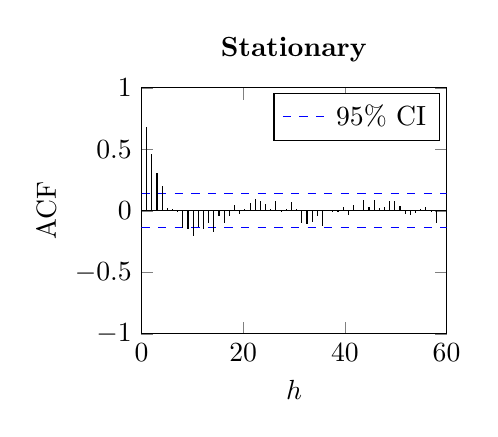
\begin{tikzpicture}
		\begin{axis}[
				ymin=-1, ymax=1,
				enlargelimits=false,
				width=0.45\textwidth,
                title=\textbf{Stationary},
				xlabel=$h$,
				ylabel=ACF,
			]
			% set pgf math constant
			\pgfmathsetmacro{\T}{200}
			\pgfmathsetmacro{\mx}{60}
			\pgfmathsetmacro{\ci}{1.96/sqrt(\T)}
			\addplot[blue, dashed, mark=none, samples=2, domain=0:\mx] {\ci};
			\addlegendentry{95\% CI};
			\addplot[blue, dashed, mark=none, samples=2, domain=0:\mx] {-\ci};
			\addplot[black, mark=none, samples=2, domain=0:\mx] {0};
			\addplot[ycomb,samples=\mx, domain=0:\mx, mark=none] {2.5*cos(\x*15)/(\x+2.5) + rand*\ci/2};
			% \addplot[ycomb, domain=0:\mx, mark=none] {cos(\x*15)};
		\end{axis}
	\end{tikzpicture}
	\hfill
	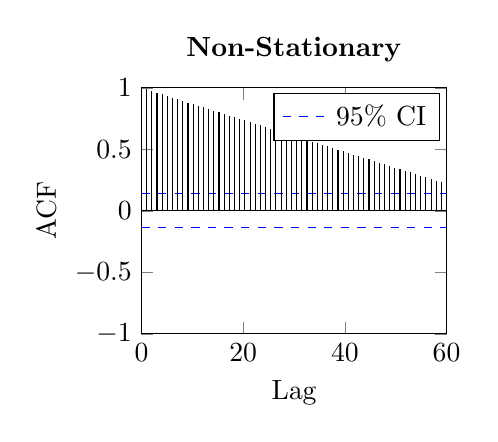
\begin{tikzpicture}
		\begin{axis}[
				ymin=-1, ymax=1,
				enlargelimits=false,
				width=0.45\textwidth,
                title=\textbf{Non-Stationary},
				xlabel=Lag,
				ylabel=ACF,
			]
			% set pgf math constant
			\pgfmathsetmacro{\T}{200}
			\pgfmathsetmacro{\mx}{60}
			\pgfmathsetmacro{\ci}{1.96/sqrt(\T)}
			\addplot[blue, dashed, mark=none, samples=2, domain=0:\mx] {\ci};
			\addlegendentry{95\% CI};
			\addplot[blue, dashed, mark=none, samples=2, domain=0:\mx] {-\ci};
			\addplot[black, mark=none, samples=2, domain=0:\mx] {0};
			\addplot[ycomb,samples=\mx, domain=0:\mx, mark=none] {1 - \x/\T*2.6};
		\end{axis}
	\end{tikzpicture}
	\caption{Correlogram of stationary and non-stationary time series.}
\end{figure}
\end{definition}

\paragraph{Variance of the sample ACF:} For a large sample size $T$, asymptotically:
\begin{equation*}
    V(\hat{\rho}_k) \approx \frac{1}{T}
\end{equation*}

The samples ACF representes the values of $\hat{\rho}_k$ for each lag $k=0,1,\dots$
The confidence bands are calculated using the asymptotic distribution for the estimator:
\begin{equation*}
    \pm \frac{1.96}{\sqrt{T}}
\end{equation*}

For each lag $k$, we can test its significance by using the plot. If
$\hat{\rho}_k$ is outside the confidence band, then we can reject the null
hypothesis $H_0:\rho_k=0$. Otherwise, we cannot reject the null hypothesis
and the theoretical ACF for this lag can be considered null.

\subsection{Partial ACF}

\begin{definition}{Partial correlation (PACF)}{PACF}\index{PACF}\index{partial autocorrelation}
    (of a stationary process) is the relationship between two variables after excluding 
    the effect of one or more independent variables.
    \tcblower
    \begin{align*}
        \phi_{11} &= \text{cor}(X_{t+1}, X_t) = \rho(1) \\
        \phi_{hh} &= \text{cor}(X_{t+h} - \hat X_{t+h}, X_t - \hat X_t),\quad h \geq 2
    \end{align*}

    \begin{note}
        Partial autocorrelation (PACF) is similar to the ACF.
    \end{note}

    \begin{example*}{}
        Consider a regression context in which $y$ is the response variable
        and $x_1,\,x_2,\,x_3$ are predictor variables. The \emph{partial correlation}
        between $y$ and $x_3$ is the correlation between the variables determined
        taking into account how both $y$ and $x_3$ are related to $x_1$ and $x_2$.
    \end{example*}

    \tcbline

    Ordinary Least Squares:
    \begin{align*}
        x_t &= \boldsymbol{\phi_{1,1}} X_{t-1} + Z_t \\
        x_t &= \phi_{1,2} X_{t-1} + \boldsymbol{\phi_{2,2}} X_{t-2} + Z_t \\
        x_t &= \phi_{1,3} X_{t-1} + \phi_{2,3} X_{t-2} + \boldsymbol{\phi_{3,3}} X_{t-3} + Z_t \\
            &\hspace{0.5em}\vdots \\
        x_t &= \phi_{1,h} X_{t-1} + \phi_{2,h} X_{t-2} + \dots + \boldsymbol{\phi_{h,h}} X_{t-h} + Z_t \\
            &\hspace{0.15em}\downarrow \\
        \textbf{PACF} &\hspace{0.1em}: \left\{
            \boldsymbol{\phi_{1,1}},\,
            \boldsymbol{\phi_{2,2}},\,\ldots\,,
            \boldsymbol{\phi_{h,h}},\,\ldots  \right\}
    \end{align*}
\end{definition}

\subsection{Autocorrelation of White Noise}

\begin{align*}
    Z_t &\sim \mathcal{WN}(\sigma_Z^2) \\
        &\sim \mathcal{N}(0,\, \sigma_Z^2)
\end{align*}
\begin{table}[H]
	\caption{Moments of white noise}%
	\label{tab:white-noise}
	\begin{tabular}{lc}
		\toprule
		Moment          & Theoretical \\ \midrule
        Mean            & 0 \\
        Autocovariance  & 0 \\
        Variance        & $\sigma_Z^2$ \\
        Autocorrelation & 0 \\
		\bottomrule
	\end{tabular}
\end{table}

\begin{figure}[H]
	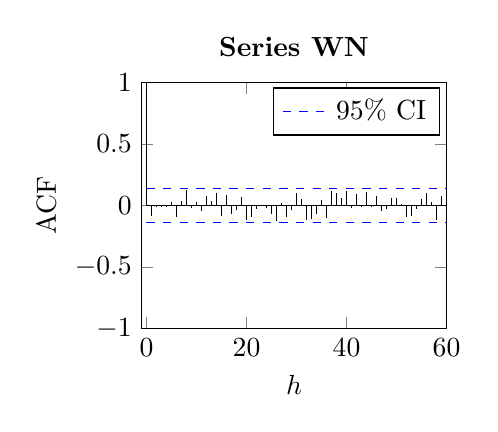
\begin{tikzpicture}
		\begin{axis}[
				ymin=-1, ymax=1,
                xmin=-1,
				enlargelimits=false,
				width=0.45\textwidth,
                title=\textbf{Series WN},
				xlabel=$h$,
				ylabel=ACF,
			]
			% set pgf math constant
			\pgfmathsetmacro{\T}{200}
			\pgfmathsetmacro{\mx}{60}
			\pgfmathsetmacro{\ci}{1.96/sqrt(\T)}
			\addplot[blue, dashed, mark=none, samples=2, domain=0:\mx] {\ci};
			\addlegendentry{95\% CI};
			\addplot[blue, dashed, mark=none, samples=2, domain=0:\mx] {-\ci};
			\addplot[black, mark=none, samples=2, domain=0:\mx] {0};
			\addplot[ycomb,samples=\mx, domain=1:\mx, mark=none] {rand*\ci*0.9};
            \addplot[ycomb] coordinates {(0,1)};
			% \addplot[ycomb, domain=0:\mx, mark=none] {cos(\x*15)};
		\end{axis}
	\end{tikzpicture}
	\hfill
	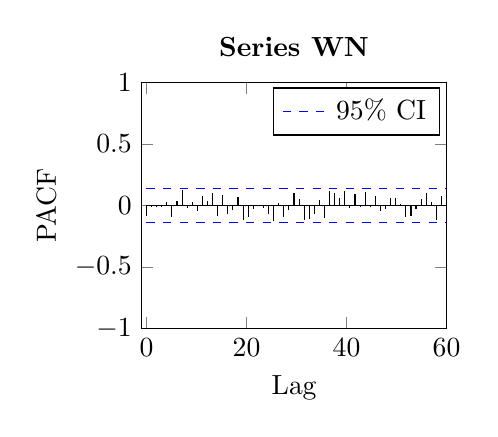
\begin{tikzpicture}
		\begin{axis}[
				ymin=-1, ymax=1,
                xmin=-1,
				enlargelimits=false,
				width=0.45\textwidth,
                title=\textbf{Series WN},
				xlabel=Lag,
				ylabel=PACF,
			]
			% set pgf math constant
			\pgfmathsetmacro{\T}{200}
			\pgfmathsetmacro{\mx}{60}
			\pgfmathsetmacro{\ci}{1.96/sqrt(\T)}
			\addplot[blue, dashed, mark=none, samples=2, domain=0:\mx] {\ci};
			\addlegendentry{95\% CI};
			\addplot[blue, dashed, mark=none, samples=2, domain=0:\mx] {-\ci};
			\addplot[black, mark=none, samples=2, domain=0:\mx] {0};
			\addplot[ycomb,samples=\mx, domain=0:\mx, mark=none] {rand*\ci*0.9};
		\end{axis}
	\end{tikzpicture}
	\caption{ACF and PACF of white noise}
\end{figure}

